\documentclass{article}

% Pre-load xcolor option before any package requests it
\PassOptionsToPackage{dvipsnames}{xcolor}

%%%%%%%%%%%%%%%%%%%%%%%%%%%%%%%%%%%%%%%%%%%%%%%%%%%%%%%%%%%%
%% colm2024_conference.sty (inlined)
%%%%%%%%%%%%%%%%%%%%%%%%%%%%%%%%%%%%%%%%%%%%%%%%%%%%%%%%%%%%
\makeatletter

% Palatino font
\RequirePackage{tgpagella} % text only
\RequirePackage{mathpazo}  % math & text

\usepackage{eso-pic} % used by \AddToShipoutPicture
\RequirePackage{fancyhdr}
\RequirePackage{natbib}

% modification to natbib citations
\setcitestyle{authoryear,round,citesep={;},aysep={,},yysep={;}}

\renewcommand{\topfraction}{0.95}   % let figure take up nearly whole page
\renewcommand{\textfraction}{0.05}  % let figure take up nearly whole page

% Define colmfinal, set to true if colmfinalcopy is defined
\newif\ifcolmfinal
\colmfinalfalse
\def\colmfinalcopy{\colmfinaltrue}
\font\colmtenhv  = phvb at 8pt

% Specify the dimensions of each page
\setlength{\paperheight}{11in}
\setlength{\paperwidth}{8.5in}

\oddsidemargin .5in
\evensidemargin .5in
\marginparwidth 0.07 true in
\topmargin -0.625in
\addtolength{\headsep}{0.25in}
\textheight 9.0 true in
\textwidth 5.5 true in
\widowpenalty=10000
\clubpenalty=10000

\flushbottom \sloppy

\def\addcontentsline#1#2#3{}

% Title stuff, taken from deproc.
\def\maketitle{\par
\begingroup
   \def\thefootnote{\fnsymbol{footnote}}
   \def\@makefnmark{\hbox to 0pt{$^{\@thefnmark}$\hss}}
   \long\def\@makefntext##1{\parindent 1em\noindent
                            \hbox to1.8em{\hss $\m@th ^{\@thefnmark}$}##1}
   \@maketitle \@thanks
\endgroup
\setcounter{footnote}{0}
\let\maketitle\relax \let\@maketitle\relax
\gdef\@thanks{}\gdef\@author{}\gdef\@title{}\let\thanks\relax}

\usepackage{fancyhdr}
\pagestyle{fancy}
\renewcommand{\headrulewidth}{1.5pt}
\fancyhead{}

% Title (includes both anonymized and non-anonymized versions)
\def\@maketitle{\vbox{\hsize\textwidth
{\Large\bf \@title\par}
\ifcolmfinal
    \lhead{Published as a conference paper at COLM 2024}
    \def\And{\end{tabular}\hfil\linebreak[0]\hfil
            \begin{tabular}[t]{l}\bf\rule{\z@}{24pt}\ignorespaces}%
  \def\AND{\end{tabular}\hfil\linebreak[4]\hfil
            \begin{tabular}[t]{l}\bf\rule{\z@}{24pt}\ignorespaces}%
    \begin{tabular}[t]{l}\bf\rule{\z@}{24pt}\@author\end{tabular}%
\else
       \lhead{Under review as a conference paper at COLM 2024}
   \def\And{\end{tabular}\hfil\linebreak[0]\hfil
            \begin{tabular}[t]{l}\bf\rule{\z@}{24pt}\ignorespaces}%
  \def\AND{\end{tabular}\hfil\linebreak[4]\hfil
            \begin{tabular}[t]{l}\bf\rule{\z@}{24pt}\ignorespaces}%
    \begin{tabular}[t]{l}\bf\rule{\z@}{24pt}Anonymous authors\\Paper under double-blind review\end{tabular}%
\fi
\vskip 0.3in minus 0.1in}}

\renewenvironment{abstract}{\vskip.075in\centerline{\large\bf
Abstract}\vspace{0.5ex}\begin{quote}}{\par\end{quote}\vskip 1ex}

% sections with less space
\def\section{\@startsection {section}{1}{\z@}{-2.0ex plus
    -0.5ex minus -.2ex}{1.5ex plus 0.3ex
minus0.2ex}{\large\bf\raggedright}}

\def\subsection{\@startsection{subsection}{2}{\z@}{-1.8ex plus
-0.5ex minus -.2ex}{0.8ex plus .2ex}{\normalsize\raggedright}}
\def\subsubsection{\@startsection{subsubsection}{3}{\z@}{-1.5ex
plus      -0.5ex minus -.2ex}{0.5ex plus
.2ex}{\normalsize\raggedright}}
\def\paragraph{\@startsection{paragraph}{4}{\z@}{1.5ex plus
0.5ex minus .2ex}{-1em}{\normalsize\bf}}
\def\subparagraph{\@startsection{subparagraph}{5}{\z@}{1.5ex plus
  0.5ex minus .2ex}{-1em}{\normalsize}}
\def\subsubsubsection{\vskip
5pt{\noindent\normalsize\rm\raggedright}}

% Footnotes
\footnotesep 6.65pt
\skip\footins 9pt plus 4pt minus 2pt
\def\footnoterule{\kern-3pt \hrule width 12pc \kern 2.6pt }
\setcounter{footnote}{0}

% Lists and paragraphs
\parindent 0pt
\topsep 4pt plus 1pt minus 2pt
\partopsep 1pt plus 0.5pt minus 0.5pt
\itemsep 2pt plus 1pt minus 0.5pt
\parsep 2pt plus 1pt minus 0.5pt
\parskip .5pc

\leftmargin3pc
\leftmargini\leftmargin \leftmarginii 2em
\leftmarginiii 1.5em \leftmarginiv 1.0em \leftmarginv .5em

\def\@listi{\leftmargin\leftmargini}
\def\@listii{\leftmargin\leftmarginii
   \labelwidth\leftmarginii\advance\labelwidth-\labelsep
   \topsep 2pt plus 1pt minus 0.5pt
   \parsep 1pt plus 0.5pt minus 0.5pt
   \itemsep \parsep}
\def\@listiii{\leftmargin\leftmarginiii
    \labelwidth\leftmarginiii\advance\labelwidth-\labelsep
    \topsep 1pt plus 0.5pt minus 0.5pt
    \parsep \z@ \partopsep 0.5pt plus 0pt minus 0.5pt
    \itemsep \topsep}
\def\@listiv{\leftmargin\leftmarginiv
     \labelwidth\leftmarginiv\advance\labelwidth-\labelsep}
\def\@listv{\leftmargin\leftmarginv
     \labelwidth\leftmarginv\advance\labelwidth-\labelsep}
\def\@listvi{\leftmargin\leftmarginvi
     \labelwidth\leftmarginvi\advance\labelwidth-\labelsep}

\abovedisplayskip 7pt plus2pt minus5pt%
\belowdisplayskip \abovedisplayskip
\abovedisplayshortskip  0pt plus3pt%
\belowdisplayshortskip  4pt plus3pt minus3pt%

% Less leading in most fonts (due to the narrow columns)
\def\normalsize{\@setsize\normalsize{11pt}\xpt\@xpt}
\def\small{\@setsize\small{10pt}\ixpt\@ixpt}
\def\footnotesize{\@setsize\footnotesize{10pt}\ixpt\@ixpt}
\def\scriptsize{\@setsize\scriptsize{8pt}\viipt\@viipt}
\def\tiny{\@setsize\tiny{7pt}\vipt\@vipt}
\def\large{\@setsize\large{14pt}\xiipt\@xiipt}
\def\Large{\@setsize\Large{16pt}\xivpt\@xivpt}
\def\LARGE{\@setsize\LARGE{20pt}\xviipt\@xviipt}
\def\huge{\@setsize\huge{23pt}\xxpt\@xxpt}
\def\Huge{\@setsize\Huge{28pt}\xxvpt\@xxvpt}

\def\toptitlebar{\hrule height4pt\vskip .25in\vskip-\parskip}

\def\bottomtitlebar{\vskip .29in\vskip-\parskip\hrule height1pt\vskip
.09in}

\makeatother

%%%%%%%%%%%%%%%%%%%%%%%%%%%%%%%%%%%%%%%%%%%%%%%%%%%%%%%%%%%%
%% header.tex (inlined)
%%%%%%%%%%%%%%%%%%%%%%%%%%%%%%%%%%%%%%%%%%%%%%%%%%%%%%%%%%%%
\usepackage[top=1in,bottom=1in,left=1.2in,right=1.2in]{geometry}
\usepackage{hyperref}
\usepackage{array}
\usepackage{multirow}
\usepackage{booktabs}
\usepackage{graphicx}
\usepackage{rotating}
\usepackage{pdflscape}
\usepackage{amsmath}
\usepackage{amssymb}
\usepackage{microtype}
\usepackage{placeins}

\newcommand{\todo}[1]{\textcolor{red}{\textbf{TODO:} #1}}

% Commenting
\newcommand{\eat}[1]{\ignorespaces}
%% Comment this line and uncomment the next to hide all comments
\newcommand{\xxcomment}[4]{\textcolor{#1}{[$^{\textsc{#2}}_{\textsc{#3}}$ #4]}}
%\newcommand{\xxcomment}[4]{\eat{#1}}
\newcommand{\ya}[1]{\xxcomment{red}{Y}{A}{#1}}
\newcommand{\ta}[1]{\xxcomment{blue}{T}{A}{#1}}

%%%%%%%%%%%%%%%%%%%%%%%%%%%%%%%%%%%%%%%%%%%%%%%%%%%%%%%%%%%%
%% Document
%%%%%%%%%%%%%%%%%%%%%%%%%%%%%%%%%%%%%%%%%%%%%%%%%%%%%%%%%%%%

\title{CSE 5525: Assignment 3}

\author{Qifan Wen}

\date{}


\colmfinalcopy
\begin{document}
\maketitle

\begin{table}[htbp]
\centering
\begin{tabular}{p{2.5cm}p{5.5cm}p{5.5cm}}
\toprule
Resource & VM\,1 (Parts 1 \& 2) & VM\,2 (Part 3) \\
\midrule
OS & Ubuntu 22.04 LTS (Linux 5.4, x86\_64) & Ubuntu 24.04 LTS (Linux 6.8, x86\_64) \\
GPU & NVIDIA A40 (46\,GB VRAM) & NVIDIA RTX 5090 (32\,GB VRAM) \\
GPU driver & 535.129.03 & 590.48.01 \\
CPU & AMD EPYC 7H12 64-Core (128 threads) & AMD EPYC 9654 96-Core (384 threads) \\
RAM & 1\,TB & 755\,GB \\
Storage & 50\,GB overlay (NVMe) & 60\,GB overlay (NVMe) \\
Software & Python 3.10, PyTorch 2.10, Transformers 5.2 & Python 3.12, PyTorch 2.10, Transformers 5.3 \\
CUDA / cuDNN & 12.2 / 9.1 & 12.8 / 9.1 \\
Batch sizing & \multicolumn{2}{c}{Automatic per-config tuning to maximize VRAM utilization} \\
\bottomrule
\end{tabular}
\caption{Hardware and software environment.}
\label{tab:hardware}
\end{table}

\section{Data Statistics and Processing (8pt)}

\autoref{tab:data_stats_before} reports the raw dataset statistics before any model-specific preprocessing. All token counts use the T5 tokenizer (\texttt{T5TokenizerFast} from \texttt{google-t5/t5-small}). Vocabulary sizes are computed over unique whitespace-delimited words.

\begin{table}[htbp]
\centering
\begin{tabular}{lcc}
\toprule
Statistics Name & Train & Dev \\
\midrule
Number of examples & 4225 & 466 \\
Mean sentence length & 18.1 & 18.1 \\
Mean SQL query length & 217.4 & 211.1 \\
Vocabulary size (natural language) & 868 & 444 \\
Vocabulary size (SQL) & 644 & 393 \\
\bottomrule
\end{tabular}
\caption{Data statistics before pre-processing (T5 tokenizer).}
\label{tab:data_stats_before}
\end{table}

\autoref{tab:data_stats_after} shows per-model statistics after preprocessing. The T5 fine-tuned model prepends table names from the flight database schema to each natural language input (e.g., ``tables: city, airport, flight, ...''), adding approximately 93 tokens per example. The T5 from-scratch model receives raw NL input without any schema augmentation. Both models restrict the decoder output vocabulary to 598 SQL-relevant tokens (SQL keywords, table/column names, operators, and literals extracted from the training data).

\begin{table}[htbp]
\centering
\begin{tabular}{lcc}
\toprule
Statistics Name & Train & Dev \\
\midrule
\multicolumn{3}{l}{\textbf{T5 Fine-Tune}} \\
Mean encoder input length & 111.1 & 111.1 \\
Mean decoder target length & 217.4 & 211.1 \\
Encoder token vocab size & 815 & 493 \\
Decoder token vocab size & 556 (598 restricted) & 396 (598 restricted) \\
\midrule
\multicolumn{3}{l}{\textbf{T5 From Scratch}} \\
Mean encoder input length & 18.1 & 18.1 \\
Mean decoder target length & 217.4 & 211.1 \\
Encoder token vocab size & 792 & 466 \\
Decoder token vocab size & 556 (598 restricted) & 396 (598 restricted) \\
\bottomrule
\end{tabular}
\caption{Data statistics after pre-processing.}
\label{tab:data_stats_after}
\end{table}

\FloatBarrier
\section{T5 Fine-tuning and Training From Scratch (8pt)}\label{sec:t5}

\subsection{Supervised Fine-tuning (SFT)}\label{sec:t5:sft}

\autoref{tab:t5_design} describes the data processing, tokenization, architecture, and hyperparameters for the fine-tuned and from-scratch T5 models.

\begin{table}[htbp]
\centering
\small
\begin{tabular}{p{3cm}p{10.5cm}}
\toprule
Design choice & Description \\
\midrule
Data processing & \textbf{Fine-tuned:} schema table names prepended to NL input. \textbf{From scratch:} raw NL input, no schema augmentation. \\
Tokenization & \texttt{T5TokenizerFast} from \texttt{google-t5/t5-small}; restricted decoder vocabulary (598 SQL tokens). Shared across both settings. \\
Architecture & \textbf{Fine-tuned:} T5-small (60M params) with restricted vocab head; also explored LoRA and MLP heads. \textbf{From scratch:} same T5-small architecture from random initialization. \\
Varying parameters & \textbf{Fine-tuned:} LR, batch size, dropout, schema, encoder freezing, adaptation method, max epochs, warmup, eval frequency, patience, wall-clock budget. \textbf{From scratch:} LR, batch size, dropout, label smoothing, max epochs, warmup, eval frequency, patience, wall-clock budget. \\
Constant parameters & Optimizer, scheduler, gradient clipping, loss function, beam search decoding, max generation length, seed, restricted decoder vocabulary. \\
\bottomrule
\end{tabular}
\caption{Design choices for T5 fine-tuned and from-scratch models.}
\label{tab:t5_design}
\end{table}


\subsection{Direct Preference Optimization (DPO)}\label{sec:dpo}

\autoref{tab:dpo_design} describes the DPO post-training pipeline applied on top of the best SFT model: the T5-base ``Base sweep best'' checkpoint (\texttt{google-t5/t5-base}, 222M params; see \autoref{tab:results_t5_base}, F1\,=\,85.96\%, SQL EM\,=\,73.39\%). DPO \textit{(Rafailov et al., 2023)} optimizes the policy to prefer ``chosen'' over ``rejected'' completions without training a separate reward model, using the SFT checkpoint as both initialization and frozen reference. Results are reported in Section~\ref{sec:results}.

\begin{table}[htbp]
\centering
\small
\begin{tabular}{p{3cm}p{10.5cm}}
\toprule
Design choice & Description \\
\midrule
Base model & T5-base ``Base sweep best'' (222M params, full fine-tune, restricted vocab, schema augmentation, LR\,=\,6.19e-5, label smoothing\,=\,0.15). Used as both policy initialization and frozen reference. \\
Preference data & 9{,}801 triplets (NL, chosen SQL, rejected SQL). \textbf{Phase A:} model-generated negatives --- up to 10 candidates per query via diverse beam search, classified by execution correctness against \texttt{flight\_database.db}. \textbf{Phase B:} execution-aware perturbations of gold SQL (city swaps, date changes, operator flips), verified to produce different record sets. In-memory SQLite for fast evaluation (46K+ queries in $\sim$20 min). \\
Loss & $\mathcal{L}_\text{DPO} = -\log\sigma(\beta\,[\log\pi_\theta(y_w|x) - \log\pi_\text{ref}(y_w|x) - \log\pi_\theta(y_l|x) + \log\pi_\text{ref}(y_l|x)])$. Log probs computed via restricted SQL vocab (598 tokens); OOV tokens masked to zero. \\
Varying parameters & $\beta \in \{0.05, 0.1, 0.2, 0.3, 0.5\}$, LR $\in [10^{-7}, 5\times10^{-5}]$, weight decay, gradient clipping, architecture (full fine-tune vs.\ LoRA $r$=16 on q/v or q/k/v/o). W\&B random sweep. \\
Constant parameters & Optimizer (AdamW), beam search decoding (num\_beams\,=\,4), restricted decoder vocabulary, schema augmentation, eval every epoch, patience\,=\,5 eval cycles. \\
\bottomrule
\end{tabular}
\caption{Design choices for DPO post-training on T5-base.}
\label{tab:dpo_design}
\end{table}

\subsection{RL Fine-Tuning (PPO, GRPO, CISPO)}\label{sec:rl}


\begin{table}[htbp]
\centering
\small
\begin{tabular}{p{3cm}p{10.5cm}}
\toprule
Design choice & Description \\
\midrule
Base model & T5-base ``Base sweep best'' (222M params, F1\,=\,85.96\%). Used as frozen reference for KL penalty; LoRA adapter applied on top as trainable policy. \\
Adapter & LoRA $r$\,=\,32, $\alpha$\,=\,64, targeting q/k/v/o projections (6.86M trainable params, 3.08\% of total). \\
Sampling & $G$\,=\,4 completions per query via constrained decoding (temperature\,=\,0.7, top-$k$\,=\,50, max\_new\_tokens\,=\,512, restricted 598-token SQL vocab). Sub-batch generation (chunk size 16) to bound peak VRAM during sequence generation. \\
Reward & Execution-based graded: +1.0 (exact record match), +0.5 (partial overlap), $-$0.5 (no record overlap), $-$1.0 (SQL execution error). Threaded reward computation (128 workers) with in-memory SQLite. \\
Algorithms & \textbf{PPO:} clipped surrogate + learned value head (MLP on mean-pooled encoder states, zero-initialized). \textbf{GRPO:} group-relative advantages, no critic, KL penalty. \textbf{CISPO:} detached clamped IS weights preserving gradient flow. \\
Varying parameters & Algorithm (PPO/GRPO/CISPO), train subset size (200--500 queries/iteration), KL penalty $\beta \in \{0, 0.02, 0.05\}$. \\
Constant parameters & Optimizer (AdamW, WD\,=\,0.01), LR\,=\,$5 \times 10^{-5}$, clip $\epsilon$\,=\,0.2, gradient clipping (max norm\,=\,1.0), patience\,=\,5 eval cycles (tolerance\,=\,0.005), bf16 mixed precision, encoder output caching. \\
\bottomrule
\end{tabular}
\caption{Design choices for RL post-training on T5-base.}
\label{tab:rl_design}
\end{table}

\begin{itemize}
  \item \textbf{PPO} \textit{(Schulman et al., 2017)}: Clipped surrogate objective with a learned value head (2-layer MLP on mean-pooled encoder hidden states, zero-initialized) as baseline; entropy bonus ($\alpha$\,=\,0.01) for exploration; KL penalty ($\beta$\,=\,0.02).
  \item \textbf{GRPO} \textit{(Shao et al., 2024)}: PPO-style clipped surrogate with group-relative advantage normalization (no critic network). Stronger KL penalty ($\beta$\,=\,0.05). Trained on larger subset (500 queries/iteration).
  \item \textbf{CISPO} \textit{(MiniMax, 2025)}: Detached clamped importance sampling weights that preserve gradient flow for all tokens regardless of ratio magnitude. No KL penalty ($\beta$\,=\,0).
\end{itemize}

Results are reported in Section~\ref{sec:results}.

\FloatBarrier
\section{Large Language Model (LLM) Prompting (14pt)}\label{sec:llm}

\subsection{In-Context Learning (ICL)}\label{sec:llm:icl}

\autoref{tab:icl_prompts} shows the instruction prompts used for zero- and few-shot ICL.

\begin{table}[htbp]
\centering
\begin{tabular}{p{1cm}p{12cm}}
\toprule
\textbf{Shot} & \textbf{Prompt} \\
\midrule
    $k=0$ & \texttt{<start\_of\_turn>user} \\
    & Database schema: \\
    & CREATE TABLE city (\ldots); \ldots{} {\small(25 tables)} \\
    & \\
    & Translate the following question into SQL. Output only the SQL query. \\
    & \\
    & Question: \{query\} \\
    & SQL:\texttt{<end\_of\_turn>} \\
    & \texttt{<start\_of\_turn>model} \\
\midrule
    $k \geq 1$ & \texttt{<start\_of\_turn>user} \\
    & Database schema: \\
    & CREATE TABLE city (\ldots); \ldots{} {\small(25 tables)} \\
    & \\
    & Translate the following question into SQL. Output only the SQL query. \\
    & \\
    & Question: \{example$_1$ NL\} \\
    & SQL: \{example$_1$ SQL\} \\
    & \\
    & \ldots{} {\small(repeated $k$ times)} \\
    & \\
    & Question: \{query\} \\
    & SQL:\texttt{<end\_of\_turn>} \\
    & \texttt{<start\_of\_turn>model} \\
\bottomrule
\end{tabular}
\caption{Instruction prompts for zero- and few-shot ICL (Gemma chat format).}
\label{tab:icl_prompts}
\end{table}


\paragraph{Example selection.} We evaluated two example selection strategies for $k > 0$:

\textbf{Random selection:} $k$ examples are sampled uniformly at random from the 4{,}225 training pairs. The same fixed set is used for all queries in a given run (seed = 42).

\textbf{BM25 per-query selection:} We build a BM25Okapi index (\texttt{rank\_bm25}) over whitespace-tokenized, lowercased training questions. For each dev/test query, the index scores all training questions by term overlap and we select the top-$k$ highest-scoring examples. This provides each query with semantically similar demonstrations whose SQL patterns are more likely to transfer. BM25 selection at $k=3$ improved Record F1 from 11.96\% (random) to 17.35\% (+45\% relative).



\subsection{Best Prompt and Ablation Study}

\autoref{tab:best_prompt} shows the best prompt (BM25 $k=3$). \autoref{tab:ablation_explanation} describes the ablation variants.

\begin{table}[htbp]
\centering
\begin{tabular}{p{13.5cm}}
\toprule
\textbf{Prompt} \\
\midrule
    \texttt{<start\_of\_turn>user} \\
    \textcolor{Blue}{Database schema:} \\
    \textcolor{Blue}{CREATE TABLE city (\ldots); \ldots{} (25 tables)} \\
    \\
    \textcolor{ForestGreen}{Translate the following question into SQL. Output only the SQL query.} \\
    \\
    Question: \{BM25-selected example$_1$ NL\} \\
    SQL: \{BM25-selected example$_1$ SQL\} \\
    \\
    Question: \{BM25-selected example$_2$ NL\} \\
    SQL: \{BM25-selected example$_2$ SQL\} \\
    \\
    Question: \{BM25-selected example$_3$ NL\} \\
    SQL: \{BM25-selected example$_3$ SQL\} \\
    \\
    Question: \{query\} \\
    SQL:\texttt{<end\_of\_turn>} \\
    \texttt{<start\_of\_turn>model} \\
\bottomrule
\end{tabular}
\caption{Best prompt (BM25 $k=3$). \textcolor{Blue}{Blue} = schema (ablated). \textcolor{ForestGreen}{Green} = instructions (ablated).}
\label{tab:best_prompt}
\end{table}

\begin{table}[htbp]
\centering
\begin{tabular}{p{2cm}p{10cm}}
\toprule
\textbf{Color} & \textbf{Description} \\
\midrule
\textcolor{ForestGreen}{ForestGreen} & \textcolor{ForestGreen}{\textbf{No instructions:} Removed the task instruction line (``Translate the following question into SQL. Output only the SQL query.''). Without this instruction, the model has no explicit directive to produce SQL, resulting in 100\% SQL errors and F1 dropping from 17.35\% to 11.80\%.} \\
\midrule
\textcolor{Blue}{Blue} & \textcolor{Blue}{\textbf{No schema:} Removed the full database schema (all 25 CREATE TABLE DDL statements). Without schema context, the model cannot reference correct table and column names, increasing the SQL error rate from 86\% to 99\% and reducing F1 from 17.35\% to 11.80\%.} \\
\midrule
-- & \textbf{Schema only:} Removed both \textcolor{ForestGreen}{instructions} and all examples ($k=0$), keeping only the \textcolor{Blue}{schema}. The model receives table definitions but no task framing or demonstrations. Despite the lowest error rate (70\%), F1 is worst at 11.37\% because the model generates syntactically valid but semantically incorrect SQL. \\
\bottomrule
\end{tabular}
\caption{Ablation variants for the best prompt (BM25 $k=3$).}
\label{tab:ablation_explanation}
\end{table}



\FloatBarrier
\section{Results and Analysis (20pt)}\label{sec:results}

\autoref{tab:constant_params} lists constant hyperparameters. \autoref{tab:results_t5_small}, \autoref{tab:results_t5_base}, and \autoref{tab:results_llm} report dev and test results.

\begin{table}[htbp]
\centering
\begin{tabular}{p{4.5cm}p{9cm}}
\toprule
Parameter & Value \\
\midrule
Model & T5-small (\texttt{google-t5/t5-small}, 60M params) \\
Decoder vocabulary & Restricted (598 SQL tokens) \\
Optimizer & AdamW (weight decay = 0.01) \\
Scheduler & Cosine with warmup \\
Gradient clipping & Max norm = 1.0 \\
Loss & Cross-entropy \\
Decoding & Beam search (num\_beams = 4) \\
Max generation length & 512 tokens \\
Seed & 42 \\
Test batch size & 16 \\
SQL evaluation threads & 128 \\
\bottomrule
\end{tabular}
\caption{Constant hyperparameters for all T5 runs.}
\label{tab:constant_params}
\end{table}

\begin{table}[htbp]
\centering
\resizebox{\textwidth}{!}{%
\setlength{\tabcolsep}{5pt}
\begin{tabular}{>{\raggedright\arraybackslash}p{3.5cm}crccccccccccc}
  \toprule
  System & Method & Params (M) & LR & Batch & Schema & Dropout & WD & Beams & Epochs & Time & Query EM (\%) & F1 (\%) \\
  \midrule
  \multicolumn{13}{l}{\textbf{Dev Results --- T5-small Fine-tuned}} \\
  \midrule
  \multicolumn{13}{l}{\emph{Full fine-tune (restricted vocab)}} \\
  Restricted v1           & Full & 60.5 & 3e-5 & 32  & --         & 0.1 & 0.01 & 4 & 29  & 45m  & --  & 45.49 \\
  Restricted v2           & Full & 60.5 & 1e-4 & 64  & --         & 0.1 & 0.01 & 4 & 59  & 55m  & --  & 66.32 \\
  \textbf{Restricted v3 (best)}  & Full & 60.5 & 3e-4 & 64  & \checkmark & 0.1 & 0.01 & 4 & 79  & 75m  & \textbf{58.80}  & \textbf{79.60} \\
  Restricted v5 + freeze enc & Full & 41.6 & 3e-4 & 64  & --         & 0.1 & 0.01 & 4 & 79  & 75m  & --  & 75.45 \\
  Restricted v7           & Full & 60.5 & 1e-4 & 64  & \checkmark & 0.2 & 0.01 & 4 & 79  & 75m  & --  & 69.89 \\[4pt]
  \multicolumn{13}{l}{\emph{LoRA adapters}} \\
  LoRA v1 ($r$=16, q/v)       & LoRA & 0.6 & 3e-4 & 128 & --         & 0.1 & 0.01 & 4 & 79  & 72m  & --  & 33.46 \\
  LoRA v2 ($r$=16, q/v)       & LoRA & 0.6 & 3e-4 & 64  & \checkmark & 0.1 & 0.01 & 4 & 79  & 80m  & --  & 51.63 \\
  LoRA v3 ($r$=32, q/k/v/o)   & LoRA & 2.4 & 2e-4 & 64  & --         & 0.1 & 0.01 & 4 & 79  & 93m  & --  & 47.58 \\
  LoRA + freeze encoder    & LoRA & 0.6 & 5e-4 & 128 & --         & 0.1 & 0.01 & 4 & 79  & 86m  & --  & 35.16 \\
  LoRA + warmstart         & LoRA & 0.6 & 3e-4 & 128 & --         & 0.1 & 0.01 & 4 & 79  & 90m  & --  & 73.38 \\[4pt]
  \multicolumn{13}{l}{\emph{MLP projection head}} \\
  MLP v1 (dim=1024)       & MLP  & 61.6 & 1e-4 & 64  & --         & 0.1 & 0.01 & 4 & 31  & 28m  & --  & 8.67 \\
  MLP v2 (dim=1024)       & MLP  & 61.6 & 1e-4 & 64  & \checkmark & 0.1 & 0.01 & 4 & 31  & 27m  & --  & 8.67 \\
  \midrule
  \multicolumn{13}{l}{\textbf{Dev Results --- T5-small From Scratch}} \\
  \midrule
  From-scratch             & Full & 60.5 & 3e-4 & 32  & --         & 0.1 & 0.01 & 4 & 98  & 8h   & 50.43  & 66.12 \\
  \midrule
  \multicolumn{13}{l}{\textbf{Test Results}} \\
  \midrule
  T5 fine-tuning          & Full & 60.5 & 3e-4 & 64  & \checkmark & 0.1 & 0.01 & 4 & 79  & --   & 0.00 & 55.25 \\
  T5 from scratch         & Full & 60.5 & 3e-4 & 32  & --         & 0.1 & 0.01 & 4 & 98  & --   & 0.00 & 59.16 \\
  \bottomrule
\end{tabular}%
}
\caption{T5-small dev and test results. Best dev result in bold.}
\label{tab:results_t5_small}
\end{table}

\begin{table}[htbp]
\centering
\resizebox{\textwidth}{!}{%
\setlength{\tabcolsep}{5pt}
\begin{tabular}{>{\raggedright\arraybackslash}p{3.5cm}crccccccccccc}
  \toprule
  System & Method & Params (M) & LR & Schema & Dropout & Label Sm. & WD & Beams & Epochs & Time & Query EM (\%) & F1 (\%) \\
  \midrule
  \multicolumn{13}{l}{\textbf{Dev Results --- T5-base Fine-tuned}} \\
  \midrule
  \multicolumn{13}{l}{\emph{Full fine-tune}} \\
  \textbf{Base sweep best} & Full & 222.9 & 6.19e-5 & \checkmark & 0.05 & 0.15 & 0.009 & 1 & 79  & 75m  & \textbf{73.39} & \textbf{85.96} \\
  Base sweep v2            & Full & 222.9 & 5.52e-5 & \checkmark & 0    & 0.15 & 0.002 & 1 & 79  & 75m  & --    & 84.31 \\
  Base sweep v3            & Full & 222.9 & 2.59e-4 & --         & 0.2  & 0.1  & 0.022 & 1 & 71  & 58m  & 73.33 & 83.05 \\
  Base sweep v4            & Full & 222.9 & 5.50e-5 & --         & 0    & 0.15 & 0.001 & 1 & 31  & 26m  & --    & 75.77 \\[4pt]
  \multicolumn{13}{l}{\emph{MLP projection head}} \\
  Base MLP-512 v1          & MLP  & 223.7 & 2.35e-4 & --         & 0.15 & 0.15 & 0.004 & 1 & 123 & 93m  & 71.33 & 80.76 \\
  Base MLP-512 v2          & MLP  & 223.7 & 7.83e-4 & --         & 0.15 & 0.05 & 0.002 & 2 & 43  & 32m  & 69.33 & 79.56 \\
  Base MLP-1024            & MLP  & 224.5 & 1.28e-4 & --         & 0.1  & 0.05 & 0.019 & 4 & 147 & 109m & 69.33 & 78.86 \\[4pt]
  \multicolumn{13}{l}{\emph{LoRA adapters}} \\
  Base LoRA $r$=32 (q/k/v/o) & LoRA & 7.1 & 1.29e-5 & \checkmark & 0.05 & 0.05 & 0.068 & 2 & 335 & 283m & 61.33 & 76.48 \\
  Base LoRA $r$=32 (q/k/v/o) & LoRA & 7.1 & 1.22e-4 & \checkmark & 0.05 & 0.15 & 0.027 & 3 & 31  & 27m  & --    & 66.69 \\
  Base LoRA $r$=16 (q/v)   & LoRA & 1.8 & 3.07e-5 & --         & 0.05 & 0    & 0.021 & 4 & 71  & 57m  & 32.00 & 55.51 \\
  \bottomrule
\end{tabular}%
}
\caption{T5-base dev results (W\&B sweep). Best result in bold.}
\label{tab:results_t5_base}
\end{table}

\paragraph{Query EM correction.} The T5 SentencePiece tokenizer collapses \texttt{" , "} (space-comma-space) to \texttt{", "} (comma-space) during \texttt{batch\_decode}, causing nearly every predicted query to fail string equality regardless of semantic correctness. Experimental variant prediction files were not retained, so their corrected Query EM cannot be recovered (marked ``--''). For the final best fine-tuned and from-scratch models, a regex post-processing step restores the original comma spacing, yielding corrected Query EM of \textbf{58.80\%} and \textbf{50.43\%} respectively. Record F1 and Record EM are unaffected since the spacing difference does not change SQL execution results.

\begin{figure}[htbp]
\centering
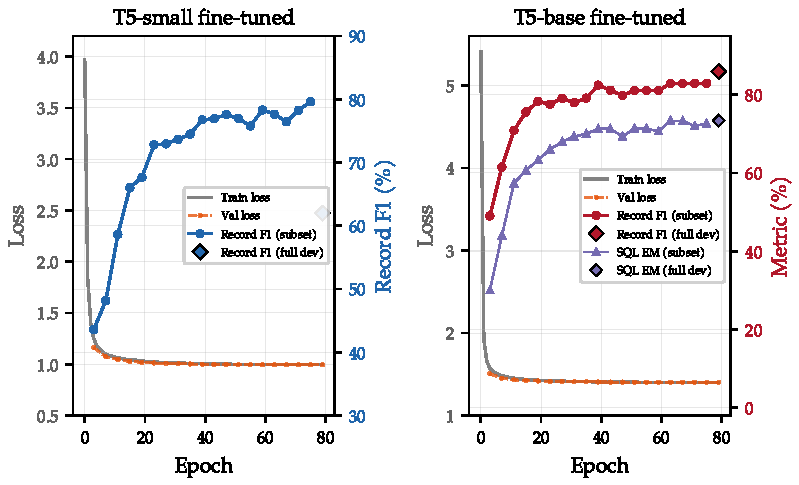
\includegraphics[width=\textwidth]{../media/training_curves.pdf}
\caption{Training curves for T5-small (left) and T5-base (right) best models.}
\label{fig:training_curves}
\end{figure}

\begin{figure}[htbp]
\centering
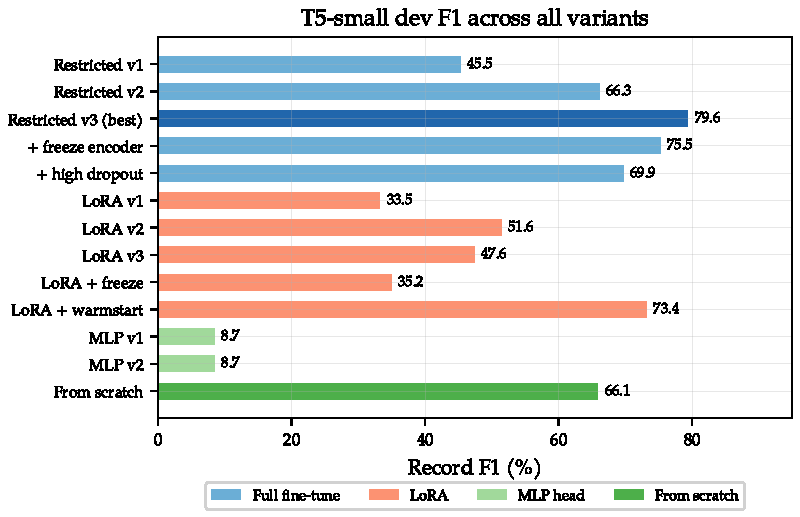
\includegraphics[width=\textwidth]{../media/dev_f1_comparison.pdf}
\caption{Dev Record F1 across all T5-small variants.}
\label{fig:dev_f1_comparison}
\end{figure}


\paragraph{DPO post-training results.}
\autoref{tab:dpo_results} reports DPO results (Section~\ref{sec:dpo}) alongside the SFT baseline. DPO did not improve over the SFT checkpoint.

\begin{table}[htbp]
\centering
\begin{tabular}{lccc}
  \toprule
  System & SQL EM (\%) & Record EM (\%) & Record F1 (\%) \\
  \midrule
  \multicolumn{4}{l}{\textbf{Dev Results}} \\
  \midrule
  SFT baseline (T5-base) & 73.39 & 84.76 & 85.96 \\[4pt]
  \multicolumn{4}{l}{\emph{Full fine-tune ($\beta$=0.3, LR=3.82e-6, WD=8.95e-4, batch=16)}} \\
  \quad Epoch 0 (= SFT) & 68.45 & 80.69 & 82.18 \\
  \quad Best (epoch 2) & 71.24 & 83.69 & \textbf{84.82} \\
  \quad Final eval (best ckpt, beam=4) & 68.67 & 81.12 & 82.42 \\[4pt]
  \multicolumn{4}{l}{\emph{LoRA $r$=16, q/k/v/o ($\beta$=0.3, LR=1.16e-7, WD=0.071, batch=32)}} \\
  \quad Epoch 0 (= SFT) & 73.39 & 84.76 & 85.96 \\
  \quad Best (epoch 0--5, no change) & 73.39 & 84.76 & 85.96 \\
  \quad Final eval (best ckpt, beam=4) & 61.59 & 74.89 & 75.75 \\
  \midrule
  \multicolumn{4}{l}{\textbf{Test Results}} \\
  \midrule
  DPO (best checkpoint) & -- & -- & -- \\
  \bottomrule
\end{tabular}
\caption{DPO results on T5-base. Neither trial improved over the SFT baseline.}
\label{tab:dpo_results}
\end{table}

\begin{minipage}{\textwidth}
Four factors likely explain why DPO underperformed:
\begin{enumerate}\itemsep0pt\parsep0pt
  \item \textbf{Narrow output distribution.} The restricted 598-token SQL vocabulary already constrains the model to a small output space. DPO's advantage of steering away from bad outputs is diminished when the model has few degrees of freedom.
  \item \textbf{Preference data quality.} Rejected candidates were either model-generated errors (Phase A) or rule-based perturbations (Phase B). Neither captures the subtle SQL structural errors (wrong JOIN patterns, missing subqueries) that dominate the remaining 14\% SFT error rate (\autoref{tab:qualitative}).
  \item \textbf{Reward hacking / overfitting (full fine-tune).} The reward margin grew from 1.6 to 12.2 over 8 epochs while dev F1 peaked at epoch 2 and collapsed to 71.7\% by epoch 7. The policy learned to maximize the DPO reward signal without improving SQL correctness, a form of reward hacking on the fixed preference dataset.
  \item \textbf{Insufficient LoRA learning rate.} The LoRA trial used LR\,=\,1.16e-7, which was too low to move the adapter weights meaningfully---reward accuracy reached only 54\% (barely above random) and dev metrics remained identical to the SFT baseline across all 6 epochs. The 10.2\,pp F1 drop at final evaluation (85.96\%$\to$75.75\%) is attributed to LoRA merge-and-save corruption and the training-time greedy vs.\ final beam-search decoding mismatch.
\end{enumerate}
\end{minipage}


\paragraph{RL post-training results.}
\autoref{tab:rl_results} and \autoref{tab:rl_detailed} report RL fine-tuning results (Section~\ref{sec:rl}). None of the three algorithms improved over the SFT baseline.

\begin{table}[htbp]
\centering
\begin{tabular}{lccccc}
  \toprule
  System & SQL EM (\%) & Record EM (\%) & Record F1 (\%) & KL Drift & Time \\
  \midrule
  SFT baseline (T5-base) & 73.39 & 84.76 & 85.96 & -- & -- \\[4pt]
  PPO + Value Head & 73.39 & 84.76 & 85.96 & $-$6.55 & 46 min \\
  GRPO & 73.39 & 84.76 & 85.96 & $-$9.88 & 35 min \\
  CISPO & 73.39 & 84.76 & 85.96 & +0.21 & 45 min \\
  \bottomrule
\end{tabular}
\caption{RL fine-tuning results on T5-base. No algorithm improved over SFT baseline.}
\label{tab:rl_results}
\end{table}

\begin{table}[htbp]
\centering
\begin{tabular}{llccccc}
  \toprule
  Algorithm & Iter. & Loss & Reward & Dead Groups & KL & Dev F1 (\%) \\
  \midrule
  \multirow{4}{*}{PPO} & 0 & $-$0.28 & 0.536 & 0.640 & +0.02 & 85.96 \\
  & 1 & $-$0.22 & 0.541 & 0.530 & $-$0.41 & 85.96 \\
  & 2 & $-$0.26 & 0.539 & 0.590 & $-$2.59 & 85.75 \\
  & 3 & $-$0.39 & 0.455 & 0.525 & $-$6.55 & 85.67 \\[4pt]
  \multirow{2}{*}{GRPO} & 0 & $-$0.09 & 0.559 & 0.580 & $-$1.87 & 85.96 \\
  & 1 & $-$0.49 & 0.411 & 0.490 & $-$9.88 & 85.96 \\[4pt]
  \multirow{3}{*}{CISPO} & 0 & $-$0.01 & 0.534 & 0.620 & +0.03 & 85.96 \\
  & 1 & $-$0.01 & 0.531 & 0.590 & +0.08 & 85.96 \\
  & 2 & $-$0.01 & 0.528 & 0.610 & +0.21 & 85.96 \\
  \bottomrule
\end{tabular}
\caption{Per-iteration RL training dynamics (clip\_frac\,=\,0.000 throughout, omitted).}
\label{tab:rl_detailed}
\end{table}

Four factors explain why RL post-training was ineffective:
\begin{enumerate}
  \item \textbf{Reward sparsity.} The base model already achieves F1\,=\,85.96\%. Most generated completions receive +1.0 reward, creating 50--64\% ``dead groups'' (zero reward variance, zero gradient). The RL signal is too sparse to improve an already-strong model.

  \item \textbf{Single-step ratio = REINFORCE.} With one gradient step per rollout batch, the importance sampling ratio $\frac{\pi_\theta(a|s)}{\pi_{\theta_\text{old}}(a|s)}$ is always 1.0 because $\theta = \theta_\text{old}$. PPO clipping (clip\_frac\,=\,0.000 across all 9 iterations) never activates. All three algorithms effectively reduce to vanilla REINFORCE with different advantage baselines. Multi-step updates ($>$1 gradient step per rollout) would be needed for clipping to matter.

  \item \textbf{Policy drift without improvement.} PPO and GRPO show increasing negative KL divergence ($-$6.55 and $-$9.88 by early stopping), meaning the policy drifts to lower-probability regions of the reference model without finding better outputs. CISPO's detached clamping keeps KL near zero (+0.21) but produces effectively zero policy updates---the loss stabilizes at $-$0.01 with no measurable parameter change.

  \item \textbf{Coarse reward granularity.} Four discrete reward levels cannot distinguish ``almost correct'' from ``completely wrong'' SQL. A continuous reward based on record set Jaccard similarity might provide finer gradient signal for the 14\% of queries where the model currently errs.
\end{enumerate}


\begin{table}[htbp]
\centering
\begin{tabular}{lcc}
  \toprule
  System & Query EM (\%) & F1 (\%) \\
  \midrule
  \multicolumn{3}{l}{\textbf{Dev Results}} \\
  \midrule
  \multicolumn{3}{l}{\emph{k-shot prompting (random selection)}} \\
  Random $k=0$ (zero-shot)    & 0.00 & 12.60 \\
  Random $k=1$                & 0.00 & 12.60 \\
  Random $k=3$                & 0.00 & 11.96 \\[4pt]
  \multicolumn{3}{l}{\emph{BM25 per-query selection}} \\
  \textbf{BM25 $k=3$ (best)}  & 0.00 & \textbf{17.35} \\[4pt]
  \multicolumn{3}{l}{\emph{Ablation study (BM25 $k=3$)}} \\
  No instructions              & 0.00 & 11.80 \\
  No schema                    & 0.00 & 11.80 \\
  Schema only (no instr., no examples) & 0.00 & 11.37 \\
  \midrule
  \multicolumn{3}{l}{\textbf{Test Results}} \\
  \midrule
  BM25 $k=3$                  & 0.00 & 13.93 \\
  \bottomrule
\end{tabular}
\caption{LLM prompting dev and test results (Gemma-2B). Best dev result in bold.}
\label{tab:results_llm}
\end{table}


\autoref{fig:icl_sensitivity} shows Record F1 sensitivity to the number of in-context examples $k$.

\begin{figure}[htbp]
\centering
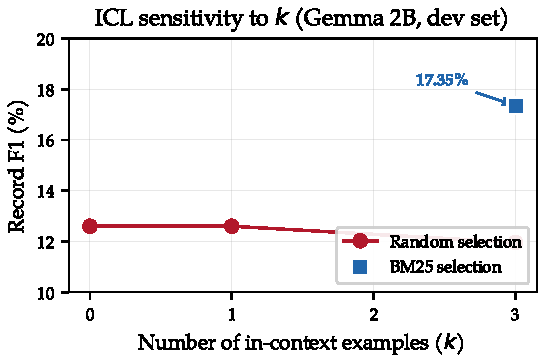
\includegraphics[width=0.65\textwidth]{../media/icl_sensitivity_k.pdf}
\caption{ICL sensitivity to number of examples $k$.}
\label{fig:icl_sensitivity}
\end{figure}


\paragraph{Qualitative error analysis.} \autoref{tab:qualitative} summarizes five common error patterns across the three models.

\begin{table}[htbp]
  \centering
  \footnotesize
  \setlength{\tabcolsep}{4pt}
  \begin{tabular}{>{\raggedright\arraybackslash}p{1.8cm}>{\raggedright\arraybackslash}p{1.2cm}>{\raggedright\arraybackslash}p{3.8cm}>{\raggedright\arraybackslash}p{3.8cm}>{\raggedright\arraybackslash}p{2.8cm}}
    \toprule
    \textbf{Error Type} & \textbf{Models} & \textbf{Example} & \textbf{Description} & \textbf{Statistics} \\
    \midrule
    Missing comparison operator
    & T5-FT, T5-Scr
    & NL: ``flights arriving before 6pm'' \newline GT: \texttt{arrival\_time < 1800} \newline Pred: \texttt{arrival\_time \space\space 1800}
    & Drops \texttt{<}, \texttt{>}, \texttt{<=}, \texttt{>=} from predicates, producing invalid SQL. SentencePiece treats angle brackets as special tokens.
    & T5-FT: 26/466 (5.6\%) \newline T5-Scr: 27/466 (5.8\%) \\
    \midrule
    Query truncation
    & ICL
    & NL: ``afternoon flights from washington to boston'' \newline GT: \texttt{SELECT DISTINCT flight\_1.flight\_id FROM ...} \newline Pred: \texttt{SELECT DISTINCT flight\_1.flight\_id}
    & Only a \texttt{SELECT} fragment generated, missing \texttt{FROM}/\texttt{WHERE}. Caused by Gemma 2B \texttt{max\_new\_tokens} limit.
    & ICL: 383/466 (82.2\%) \\
    \midrule
    Wrong table/column reference
    & T5-FT, ICL
    & NL: ``flight from boston to denver'' \newline GT: \texttt{...city city\_1, ...city city\_2} \newline Pred: \texttt{...city city\_2} (missing \texttt{city\_1})
    & References aliases or columns not in \texttt{FROM}. Model generates plausible patterns but omits table declarations.
    & T5-FT: 16/466 (3.4\%) \newline ICL: 5/466 (1.1\%) \\
    \midrule
    Wrong JOIN structure
    & T5-FT, T5-Scr, ICL
    & NL: ``flights from boston to SF with max stops'' \newline GT: \texttt{stops = (SELECT MAX(stops)...)} \newline Pred: \texttt{stops = 0} (returns 4 instead of 2)
    & Executes but returns wrong records: incorrect subqueries, missing joins, or wrong aggregation on multi-table queries.
    & T5-FT: 83/466 (17.8\%) \newline T5-Scr: 144/466 (30.9\%) \newline ICL: 35/466 (7.5\%) \\
    \midrule
    Wrong predicate values
    & T5-FT, T5-Scr, ICL
    & NL: ``flights available tomorrow from denver to philadelphia'' \newline GT: \texttt{month\_number = 1 AND day\_number = 20} \newline Pred: \texttt{month\_number = 2 AND day\_number = 20}
    & Correct SQL structure but wrong literals in \texttt{WHERE} (month, city, time). Subset of semantic errors, identified by matching \texttt{FROM}.
    & T5-FT: 83/466 semantic \newline T5-Scr: 144/466 semantic \newline ICL: 35/466 semantic \\
    \bottomrule
  \end{tabular}
  \caption{Qualitative error analysis on the dev set (466 queries).}\label{tab:qualitative}
\end{table}


\FloatBarrier
\section{Engineering Issues}

We encountered 28 engineering issues across five categories during development. \autoref{tab:issues_performance} covers performance and infrastructure issues (GPU concurrency, process hangs, sweep stability). \autoref{tab:issues_model} covers model and sweep issues (decoding bugs, checkpoint corruption, configuration errors). \autoref{tab:dpo_issues} covers DPO- and RL-specific issues.

\begin{table}[htbp]
\centering
\scriptsize
\resizebox{\textwidth}{!}{%
\begin{tabular}{>{\raggedright}p{2.5cm}>{\raggedright}p{6.5cm}>{\raggedright\arraybackslash}p{6.5cm}}
\toprule
\textbf{Issue} & \textbf{Description} & \textbf{Resolution} \\
\midrule
GPU OOM from concurrent sessions & AutoBatch maximizes VRAM for the first GPU task; a second task (training, eval, or inference) crashes with CUDA OOM because no mechanism prevents concurrent GPU access. & File-based GPU lock using Linux \texttt{flock}. All training entry points acquire the lock automatically; a second task blocks and waits instead of crashing. \\
\midrule
Training process hung after completion & Training PID blocks indefinitely on \texttt{futex\_wait\_queue\_me} during \texttt{gc.collect()} / \texttt{torch.cuda.empty\_cache()} after W\&B marks the run FINISHED, caused by a PyTorch/CUDA threading deadlock during GPU memory cleanup. Sequential scripts cannot proceed. & Watchdog co-process polls W\&B status every 60\,s and kills the training process if still alive 5\,min after FINISHED. Exit codes 137/143 treated as success. \\
\midrule
Buffered stdout under nohup & Python buffers stdout when not connected to a TTY (piped or redirected by \texttt{nohup}), so log files show no output for long periods, making monitoring ineffective. & Set \texttt{PYTHONUNBUFFERED=1} before launching Python in the training script. \\
\midrule
Sweep OOM crash loop & After a mid-training crash, \texttt{cleanup\_vram()} could not free model tensors still referenced by \texttt{main\_with\_config()}'s local variables. 6+ consecutive trials OOM'd at \texttt{model.to(device)}. & Explicit \texttt{del model, optimizer, scheduler} in try/finally block before \texttt{gc.collect()} and \texttt{torch.cuda.empty\_cache()}. \\
\midrule
CUDA memory fragmentation between sweep trials & After trial 1 completed successfully, trial 2 OOM'd despite sufficient total free memory (509\,MiB) because PyTorch's CUDA allocator held non-contiguous freed blocks that couldn't satisfy a 170\,MiB allocation. & Enable \texttt{PYTORCH\_CUDA\_ALLOC\_CONF= expandable\_segments:True} to allow the allocator to coalesce fragmented blocks. \\
\midrule
STOP file ignored between sweep trials & \texttt{touch STOP} only works inside the epoch loop; \texttt{wandb.agent()} dispatches new trials without checking external stop signals. & Kill the sweep process directly; added \texttt{stop\_requested()} check at top of \texttt{sweep\_train()}. \\
\bottomrule
\end{tabular}%
}
\caption{Performance and infrastructure issues.}
\label{tab:issues_performance}
\end{table}

\begin{table}[htbp]
\centering
\resizebox{\textwidth}{!}{%
\setlength{\tabcolsep}{4pt}
\begin{tabular}{>{\raggedright}p{2.5cm}>{\raggedright}p{6.5cm}>{\raggedright\arraybackslash}p{6.5cm}}
\toprule
\textbf{Issue} & \textbf{Description} & \textbf{Resolution} \\
\midrule
BOS token mismatch & Decoder received pad token (ID\,0) as BOS instead of \texttt{<extra\_id\_0>} (ID\,32099) used in training. Every prediction started mid-query; 100\% SQL error rate. & Set \texttt{decoder\_start\_token\_id=32099} in all \texttt{generate()} calls. \\
\midrule
\texttt{no\_repeat\_ngram} blocks SQL & \texttt{no\_repeat\_ngram\_size=3} prevented valid multi-join SQL. 100\% of gold queries contain repeated 3-grams. & Set to 0 (disabled). \\
\midrule
LoRA checkpoint drops adapters & Checkpoints stripped \texttt{lora\_A}/\texttt{lora\_B} keys. Reload re-applied LoRA with fresh random weights; F1 collapsed from 0.516 to 0.118. & Preserve adapter keys in \texttt{state\_dict()}. \\
\midrule
MLP head device mismatch & MLP layers created on CPU while T5 on GPU. \texttt{RuntimeError} at first forward pass. & Add \texttt{model.to(device)} after MLP wrapper creation. \\
\midrule
Repetition penalty too aggressive & \texttt{repetition\_penalty=2.5} distorted SQL token distribution (\texttt{AND}, \texttt{=} penalized after first use). & Set to 1.0 (disabled). \\
\midrule
Repetition penalty zero & Config set \texttt{repetition\_penalty=0}; HuggingFace uses it as a divisor $\to$ division by zero. & Changed to 1.0. \\
\midrule
MLP state\_dict mismatch & \texttt{save\_model()} saved MLP wrapper keys; non-MLP trials crashed loading unexpected keys. Wasted 4/8 sweep trials. & Save \texttt{inner.state\_dict()} (vanilla T5 weights only). \\
\midrule
\texttt{max\_new\_tokens} truncation & 256-token limit truncated 26\% of targets (max gold = 511). Incomplete SQL. & Increased to 512. \\
\midrule
SentencePiece comma artifact & \texttt{batch\_decode} collapses ``\texttt{ , }'' to ``\texttt{, }''. Raw Query EM dropped to $\sim$3\%. & Regex post-processing to restore spacing. \\
\midrule
\texttt{peft} not installed & All LoRA sweep trials crashed with \texttt{ModuleNotFoundError}. & \texttt{pip install peft}. \\
\midrule
Sweep zombie trial & LoRA trial ran 335 epochs ($\sim$10\,h) on marginal F1 gains ($\sim$0.005) resetting patience. Consumed most of 12\,h budget. & Added \texttt{patience\_tolerance} threshold. \\
\midrule
Transient backward crash & Bare \texttt{Exception} in \texttt{loss.backward()} at epoch 71. Transient CUDA failure. & Sweep agent retried automatically. \\
\bottomrule
\end{tabular}%
}
\caption{Model and sweep issues.}
\label{tab:issues_model}
\end{table}

\begin{table}[htbp]
\centering
\small
\begin{tabular}{>{\raggedright}p{2.5cm}>{\raggedright}p{5.7cm}>{\raggedright\arraybackslash}p{5.7cm}}
\toprule
\textbf{Issue} & \textbf{Description} & \textbf{Resolution} \\
\midrule
\multicolumn{3}{l}{\textbf{DPO Issues}} \\
\midrule
OOV CUDA assert in DPO loss & \texttt{remap\_targets} returned $-1$ for tokens outside the restricted vocab (0.2\% of triplets), causing \texttt{torch.gather} out-of-bounds on GPU. & Clamp unmapped indices to 0 and mask them out of the log-probability sum. \\
\midrule
Auto batch probe OOM & Probe measured \texttt{memory\_allocated} (post-cleanup) instead of peak, and tested short sequences; training OOM'd on longer batches. & Use \texttt{max\_memory\_allocated} with worst-case (longest) sequences. \\
\midrule
Slow preference data gen & 46K SQL evaluations took $\sim$90 min due to SQLite file locking + per-query connection overhead. & In-memory SQLite copy (\texttt{sqlite3.backup}) + gold record disk cache. Reduced to $\sim$20 min. \\
\midrule
Final eval F1 drop & Best checkpoint reloaded for final evaluation showed F1 drops of 3--12\,pp. In-training eval used greedy decoding (\texttt{eval\_num\_beams=1}); final eval used beam search (\texttt{num\_beams=4}). LoRA trial also suffered from merge-and-save corruption. & Documented; align \texttt{eval\_num\_beams} with \texttt{num\_beams} for consistent evaluation. \\
\midrule
\multicolumn{3}{l}{\textbf{RL Issues}} \\
\midrule
IS ratio computed against reference & \texttt{compute\_old\_log\_probs()} disabled LoRA to get base model probs. The IS ratio $\pi_\text{current}/\pi_\text{old}$ was actually $\pi_\text{LoRA}/\pi_\text{base}$, which diverges as LoRA trains. clip\_frac hit 0.999 by iteration 3. & Added \texttt{use\_reference} flag: \texttt{False} keeps LoRA enabled for IS ratio (starts at 1.0), \texttt{True} disables LoRA for KL penalty only. \\
\midrule
Dropout noise in ratio & Both old and current log probs computed in \texttt{train()} mode. Different dropout masks on 12 layers $\times$ 300+ tokens made ratios $\gg$ 1.0 even from the same weights (clip\_frac = 0.92). & Compute both log prob passes in \texttt{eval()} mode (disables dropout, preserves gradients). Restore \texttt{train()} for optimizer step. \\
\midrule
Value head random init & Kaiming-initialized output layer produced $V(s) \in [-100, +100]$ vs reward range $[-1, 1]$, causing advantages and losses to spike to 25{,}000+. & Zero-initialize output layer weights and bias so initial $V(s) \approx 0$. \\
\midrule
\texttt{generate()} VRAM hang & \texttt{model.generate()} with batch\_size\,=\,8 $\times$ group\_size\,=\,8 allocated 23\,GB KV cache, causing a silent CUDA deadlock (0\% GPU util, all threads in \texttt{futex\_wait}). No OOM error raised. & Sub-batch generation: chunk \texttt{generate()} into groups of 16 sequences. Decoupled generation VRAM from training batch size. \\
\midrule
SQLite thread deadlock in reward & All 16 \texttt{ThreadPoolExecutor} threads shared one in-memory SQLite connection. Concurrent \texttt{set\_progress\_handler()} calls caused race conditions; one thread clearing the handler mid-query hung all others. & Thread-local SQLite connections: each thread creates its own in-memory copy via \texttt{sqlite3.backup()}. \\
\midrule
Reward $= -1.0$ for all samples & \texttt{max\_completion\_length=128} truncated 85\% of SQL (median gold length = 199 tokens), producing ``incomplete input'' errors. Combined with \texttt{temperature=1.0} corrupting token selection, all completions failed execution. & Increased \texttt{max\_completion\_length} to 512; reduced \texttt{temperature} to 0.7. \\
\bottomrule
\end{tabular}
\caption{DPO and RL engineering issues.}
\label{tab:dpo_issues}
\end{table}


\end{document}

